\documentclass[10pt]{article}
%PACKEGE%
\usepackage[italian]{babel}
\usepackage{amsmath,amsfonts,amssymb,mathtools,ulem,latexsym, graphicx}
\usepackage[utf8x]{inputenc}
\usepackage[makeroom]{cancel}
\usepackage[margin=1.0in]{geometry}
\usepackage{tikz}
\usetikzlibrary{arrows}
\usepgflibrary{arrows}
%DOCUMENTO%
\title{Fondamenti Matematici per l'Informatica: Teoremi e Dimostrazioni}
\author{Aymane Chabbaki}
\date{II semestre 2018/2019}

\begin{document}
\maketitle
\tableofcontents
\newpage
%-------------------------------------------------------------------%
%-------------------------------------------------------------------%
%-------------------------------------------------------------------%
\section{Insiemi}
\subsection{Teorema del Buon ordinamento}
\textsc{Enunciato:}
\begin{itemize}
\item
L'insieme totalmente ordinato $(\mathbb{N}, \leq)$ è \textbf{ben ordinato}.
\end{itemize}
\textsc{Dimostrazione:}
\begin{itemize}
\item
Sia $A$ un sottoinsieme di $\mathbb{N}$ senza minimo. 
\item
Devo provare che $A = \varnothing $ o equivalentemente $B := \mathbb{N} \setminus \! A = \mathbb{N}$
\item
Proviamo per induzione che vale $\forall n \!\in\! \mathbb{N}$, $ \underbrace{\{0,1,\dots,n\} \subset B}_{P(n)} $
\item
$n=0$ (\textbf{base dell'induzione})
\begin{itemize}
\item
$\{0\} \subset B \Longleftrightarrow 0 \in B$
\item
Questo è vero, cioè $0 \!\in\! B$, altrimenti se $0 \in \mathbb{N} \setminus \! B = A \Longrightarrow 0 = min(A)$ e questo è impossibile perchè $A$ non ha minimo.
\item
Dunque $0 \!\in\! B$
\end{itemize}
\item
$n \Longrightarrow n+1$
\item
Assumiamo che  $\{0,1,\dots,n\} \subset B$ per qualche $n \!\in \!\mathbb{N}$ (\textbf{ipotesi induttiva})
\item
Devo provare che anche $\{0,1,\dots,n, n+1\} \subset B$
\begin{itemize}
\item
$n+1 \not \in A$ altrimenti $(n+1) = min(A)$ visto che tutti gli altri elementi precedenti stanno in $B$.
\item
Questo è impossibile perchè $A$ non ha minimo.
\item
Dunque $n+1 \in B \Longrightarrow \{0,1,\dots,n, n+1\} \subset B $
\end{itemize}
\item
$A$ è vuoto e $\mathbb{N}$ è \textbf{ben ordinato}.
\item
$C.V.D.$
\end{itemize}
%-------------------------------------------------------------------%
\subsection{Seconda forma del Principio di Induzione}
\textsc{Enunciato:}
\begin{itemize}
\item
Sia $\displaystyle{\{P(n)\}_{n \in \mathbb{N}}}$ una famiglia di affermazioni (\textbf{proposizioni}) indicizzate su $\mathbb{N}$.
\item
Supponiamo che:
\begin{enumerate}
\item
$P(0)$ è vera (\textbf{base dell'induzione}).
\item
$\forall n > 0$, ($P(k)$ è vera $\forall k < n$) $\implies$ ($P(n)$ è vera)
\end{enumerate}
\item
Allora $P(n)$ è vera $\forall n \!\in\! \mathbb{N}$.
\end{itemize}
\textsc{Dimostrazione:}
\begin{itemize}
\item
$A := \{n \!\in\!\mathbb{N} \;|\; P(n)$ è falsa$\}$
\item
Supponiamo per assurdo che $A \neq \varnothing$.
\item
Grazie al Teorema di buon ordinamento di $(\mathbb{N}, \leq)$ si ha che $\exists n := min(A)$
\item
Chiaramente $0 \not \in A$ poichè $P(0)$ è vera.
\item
Inoltre se $k<n$, allora  $k \not \in A$ in quanto $n= min(A)$, ma allora dalla (2) segue che $P(n)$ è vera e quindi $n \not \in A$, contraddicendo il fatto che $n \in A$.
\item
$C.V.D.$
\end{itemize}
\newpage
%-------------------------------------------------------------------%
%-------------------------------------------------------------------%
%-------------------------------------------------------------------%
\section{Numeri}
\subsection{Divisione Euclidea}
\textsc{Enunciato:}
\begin{itemize}
\item
Siano $n,m \in \mathbb{Z}$ con $m \neq 0$, allora esistono unici $q,r \in \mathbb{Z}$ tali che:
\[
\begin{cases}
n=m \cdot q + r \\
0 \leq r < |m|
\end{cases}
\]
\end{itemize}
\textsc{Dimostrazione Esistenza:}
\begin{itemize}
\item
Supponiamo che $n \geq 0$ e $m > 0$:
\begin{itemize}
\item
Procediamo per induzione su $n \geq 0$ per dimostrare che se $m \!>\! 0$ allora $\exists \, q,r \in \mathbb{N}$, tale che: $\begin{cases} n = m \cdot q + r \\ 0 \leq r < m \end{cases}$
\item
$n=0$ (\textbf{base dell'induzione}).
$$\begin{cases} n = 0 = \,? \cdot m \, + \, ? = 0 \cdot m + 0 \\ 0 \leq 0 < m \end{cases}$$
\item
Dunque basta prendere $n = 0$ e $r=0$.
\item
Supponiamo ora che $n > 0$, $k < m \implies n$.
\item
Assumiamo l'asserto vero $\forall \, k < n$, cioè $\exists \, q', r' \in \mathbb{N} \,\, tc. \,\, k = q' \cdot m + r'$ e $0 \leq r' < m$ (\textbf{ipotesi induttiva}).
\item
Se $n < m$ basta prendere $q = 0$ e $r = n$.
\item
Se $n \geq m$ poniamo $k := n - m < n \implies 0 \leq k < n$.
\item
Grazie all'ipotesi induttiva esistono $q', r' \in \mathbb{N} \,\,tc:\begin{cases} k = q' \cdot m + r' \\ 0 \leq r' < m \end{cases}$
\item
$n-m = k = q' \cdot m + r'$, $0 \leq r' < m$
\item
Ma allora $n = k + m = m \cdot q + r' + m = (q' + 1)m + r'$, vale anche per $n \implies \forall \,n \geq 0$ è vera.
\end{itemize}
\item
Supponiamo ora $n < 0$ e $m > 0$:
\begin{itemize}
\item
Per il caso precedente si ha che esistono $q,r \in \mathbb{Z}$ tali che: $\begin{cases} -n = q \cdot m + r \\ 0 \leq r < n \end{cases}$
\item
E quindi $n= (-q)m - r$.
\item
Se $r = 0$ allora $-q$ è il quoziente e $r=0$ è il resto.
\item
Se $0<r<m$:
$$n = (-q)m - m + m - r = (-q -1)m + (m-r)$$
$$\textrm{con } 0<m-r<m = |m|$$
\end{itemize}
\item
Sia $n \in \mathbb{Z}$ e $m < 0$:
\begin{itemize}
\item
Per i due casi precedenti esistomo $q,r \in \mathbb{Z}$ tali che 
$$n = q(-m) + r = (-q)m + r$$
$$\textrm{con } 0<r<-m = |m|$$
\end{itemize}
\end{itemize}
%-------------------------------------------------------------------%
\textsc{Dimostrazione Unicità:}
\begin{itemize}
\item
Supponiamo esistano $q, q', r, r' \in \mathbb{N}$ tale che: $q' \cdot m + r' = n = q \cdot m + r $ con $0 \leq r'$, $r<m$
\item
Cioè:
\begin{equation}
\begin{split}
q' \cdot m + r' &= q \cdot m + r \\
q' \cdot m - q \cdot m &= r - r' \\
(q' - q) \cdot m &= r - r'
\notag
\end{split}
\end{equation}
\item
Supponiamo che $r' \geq r$ e passando ai moduli si ha:
\begin{equation}
\begin{split}
 |q' - q| \, m &= |r-r'| = r-r' < m \\
 |q' - q| \, |m| < |m| & \Longleftrightarrow |q' - q| \, m < m \\
 & \Longleftrightarrow |q' - q| < 1 \\
 & \Longleftrightarrow |q' - q| = 0 \\
 & \Longleftrightarrow q' - q = 0 \\
 & \Longleftrightarrow q' = q 
 \notag
\end{split}
\end{equation}
\item
Visto che $q' = q$ si ha che: $$\cancel{q' \cdot m} + r' = n = \cancel{q \cdot m} + r \implies r' = r$$
\item
$C.V.D.$
\end{itemize}
%-------------------------------------------------------------------%
\subsection{Rappresentazione binaria dei naturali in base arbitraria}
\textsc{Enunciato:}
\begin{itemize}
\item
Sia $b \in \mathbb{N}$, $b \geq 2$. 
\item
Allora ogni $n\in \mathbb{N}$ è rappresentabile, in \textbf{modo unico}, in base $b$. Ovvero $\exists \,! \{\varepsilon_i\}_{i \in \mathbb{N}}$ tale che $\varepsilon_{i \in I_b} \forall i \in \mathbb{N}$ la successione $\{\varepsilon_i\}_{i \in \mathbb{N}}$ è definitivamente nulla e vale:
$$ n = \displaystyle{\sum_{i=0}^{\infty} \varepsilon_i \cdot b^i = (\dots \cdot \varepsilon_2 \cdot \varepsilon_1 \cdot \varepsilon_0)_b}$$
\end{itemize}
\textsc{Dimostrazione Esistenza:}
\begin{itemize}
\item
Procediamo per induzione (2° forma) su $n$:
\begin{itemize}
\item
$n=0$ (\textbf{base dell'induzione})
\item
Poniamo $\varepsilon_i = 0 \,\, \forall i \in \mathbb{N}$. Vale:
\begin{enumerate}
\item
$\{\varepsilon_i\}_{i \in \mathbb{N}}$ è definitivamente nulla.
\item
$\varepsilon_i = 0 \in I_b \,\, \forall i \in \mathbb{N}$
\item
$n=0 = \displaystyle{\sum_{i \in \mathbb{N}}^{\infty} 0 \cdot b^i}$
\end{enumerate}
\item
$n>0$, $\forall k < n \implies n$
\item
Eseguiamo la divisione euclidea di $n$ per $b$:
$$n = q \cdot b + r, \quad q,r \in \mathbb{N}$$
$$0 \leq r < b \quad (\Longleftrightarrow r \in I_b)$$
\item
Dico che $q<n$:
\begin{itemize}
\item
Se $q=0$, allora $q = 0 < n$
\item
Se $q \neq 0$ allora: $0 < q < q \cdot b + r = n$, quindi segue che $q < n$
\end{itemize}
\item
Applicando l'ipotesi induttiva con $k = q$ si ha quindi che esiste $\{\zeta_i\}_{i \in \mathbb{N}}$ con $\zeta_{i \in I_b}$ definitivamente nulla e $q = \displaystyle{\sum_{i=0}^{\infty} \zeta_i \cdot b^i}$
\item
Si ha:
\begin{equation}
\begin{split}
n = q \cdot b + r &= \displaystyle{\sum_{i=0}^{\infty} \left(\zeta_i \cdot b^i\right) \cdot b + r} \\
&= r + \displaystyle{\sum_{i=0}^{\infty} \zeta_i \cdot b^{i+1}} \\
&= r + \displaystyle{\sum_{i=1}^{\infty} \zeta_{i-1} \cdot b^{i}}
\notag
\end{split}
\end{equation}
$\implies r \in I_b$ e $\zeta_{i-1} \in Ib \,\, \forall i \geq 1$
\item
Definiamo:
\begin{itemize}
\item
$\varepsilon_0 = r$
\item
$\varepsilon_i = \zeta_{i-1} \,\, \forall i \geq 1$
\end{itemize}
$\implies \{\varepsilon_i\}_{i \in \mathbb{N}}$ è definitivamente nulla e $\varepsilon_{i \in I_b} \forall i \in \mathbb{N}$
$\implies n = \varepsilon_0 + \displaystyle{\sum_{i=1}^{\infty} \varepsilon_i \cdot b^i = \sum_{i=0}^{\infty} \varepsilon_i \cdot b^i}$
\end{itemize}
\item
Dunque esiste una scrittura in base $b$ $\forall n \in \mathbb{N}$
\item
$C.V.D.$
\end{itemize}
%-------------------------------------------------------------------%
\textsc{Dimostrazione Unicità:}
\begin{itemize}
\item
Sia $n \in \mathbb{N}$ tale che:
\begin{enumerate}
\item
$\exists \, \{\varepsilon_i\}_{i \in \mathbb{N}}$ tale che:
\begin{itemize}
\item
$\{\varepsilon_i\}_{i \in \mathbb{N}}$ è definitivamente nulla
\item
$\varepsilon_{i \in I_b} \,\, \forall i \in \mathbb{N}$
\item
$n = \displaystyle{\sum_{i \in \mathbb{N}} \varepsilon_i \cdot b^i}$
\end{itemize}
\item
$\exists \, \{ \varepsilon^{'}_{i} \}_{i \in \mathbb{N}}$ tale che:
\begin{itemize}
\item
$\{\varepsilon^{'}_i \}_{i \in \mathbb{N}}$ è definitivamente nulla.
\item
$\varepsilon^{'}_{i \in I_b} \,\, \forall i \in \mathbb{N}$
\item
$n = \displaystyle{\sum_{i \in \mathbb{N}} \varepsilon^{'}_i \cdot b^i}$
\end{itemize}
$\implies \varepsilon_i = \varepsilon^{'}_i \quad \forall i \in \mathbb{N}$
\end{enumerate}
\item
Procediamo per induzione su $n \in \mathbb{N}$ e dimostriamo che la rappresentazione di $n$ in base $n$ è unica.
\begin{itemize}
\item
$n=0$ (\textbf{base dell'induzione})
$$ \sum_{i \in \mathbb{N}} \varepsilon_i \cdot b^i = \quad 0 \quad = \sum_{i \in \mathbb{N}} \varepsilon^{'}_i \cdot b^i $$
$$ \varepsilon_i \cdot b = 0 \,\, \forall i \in \mathbb{N} \quad \quad \quad \varepsilon^{'}_i \cdot b = 0 \,\, \forall i \in \mathbb{N} $$
$$\!\!\!\!\varepsilon_i = 0 \,\,\forall i \quad \quad \quad \quad \quad \quad \varepsilon^{'}_i = 0 \,\, \forall i$$ 
$\implies \varepsilon_i = \varepsilon^{'}_i \,\, \forall i$
\item
$n>0$, $\forall k < n \implies n$
$$ \sum_{i \in \mathbb{N}} \varepsilon_i \cdot b^i = \quad n \quad = \sum_{i \in \mathbb{N}} \varepsilon^{'}_i \cdot b^i $$
$$ \varepsilon_0 + \displaystyle{\sum_{i=0}^{\infty} \varepsilon_i \cdot b^i \quad \quad \varepsilon^{'}_0 + \sum_{i=0}^{\infty} \varepsilon^{'}_i \cdot b^i}$$
$$\displaystyle{\varepsilon_0 + \underbrace{\left(\sum_{i=1}^{\infty} \varepsilon_i \cdot b^{i-1} \right) \cdot b}_{q} \quad \quad \varepsilon^{'}_0 + \underbrace{\left(\sum_{i=1}^{\infty} \varepsilon^{'}_i \cdot b^{i-1} \right) \cdot b}_{q^{'}}}$$
\item
Siccome la divisione euclidea è unica $q = q' < n \implies \varepsilon_0 = \varepsilon^{'}_0$
$$ \displaystyle{\sum_{i = 1}^{\infty} \varepsilon_i \cdot b^{i -1} = \quad q \quad = \sum_{i = 1}^{\infty} \varepsilon^{'}_i \cdot b^{i -1}  \quad < n}$$
$$\!\!\!\!\!\!\!\!\!\!\!\!\!\!\!\!\sum_{i = 0}^{\infty} \varepsilon_{i-1} \cdot b^{i} = \quad q \quad = \sum_{i = 0}^{\infty} \varepsilon^{'}_{i-1} \cdot b^{i}$$
\item
Per ipotesi induttiva $\varepsilon_{i+1} = \varepsilon^{'}_{i+1} \,\,\forall i \geq 0$
\item
$C.V.D.$
\end{itemize}
\end{itemize}
%-------------------------------------------------------------------%
\subsection{Esistenza ed unicità del Massimo Comune Divisore}
\textsc{Enunciato:}
\begin{itemize}
\item
Siano $n,m$ due numeri \textbf{interi} non entrambi nulli. 
\item
Si dice che un numero naturale $d$ è il \textbf{massimo comune divisore} tra $n$ e $m$ se soddisfa:
\begin{enumerate}
\item
$d \,|\, n$ e $d \,|\, m$ (\textbf{comune divisore})
\item
Se $c \in \mathbb{Z}$ tale che $c \,|\, n$ e $c \,|\, m$ allora $c \,|\, d$ (se esiste, allora $d$ è il massimo tra i divisore comuni tra $n$ e $m$)
\end{enumerate}
\item
Se un tale $d$ esiste, allora è \textbf{unico} (è il massimo comune divisore) e si indica con $(n,m) = d$
\end{itemize}
\textsc{Dimostrazione Unicità:}
\begin{itemize}
\item
Supponiamo l'esistenza, e quindi che valgano le proprietà della definizione.
\item
Siano $d$ e $d'$ due massimi comuni divisori di $n$ e $m$. Allora:
\[
d \,|\, d'
\begin{cases}
(1) \textrm{ con } d \\
(2) \textrm{ con } d'
\end{cases}
\]
\[
d' \,|\, d
\begin{cases}
(1) \textrm{ con } d'\\
(2) \textrm{ con } d
\end{cases}
\]
\item
$d=\pm d'$ ma visto che sono numeri naturali si ha che $d = d'$
\item
$C.V.D.$
\end{itemize}
\newpage
\textsc{Enunciato Esistenza MCD:}
\begin{itemize}
\item
Dati qualunque $n,m \in \mathbb{Z}$ non entrambi nulli, \textbf{esiste sempre}, ed è \textbf{unico} il massimo comune divisore tra $n$ e $m$.
\item
Dati $n,m \in \mathbb{Z}$ vale $n \,|\, m \Longleftrightarrow n \,|\, -m \Longleftrightarrow -n \,|\, m \Longleftrightarrow -n \,|\, -m$
\end{itemize}
\textsc{Dimostrazione Esistenza:}
\begin{itemize}
\item
Possiamo supporre che $n \geq 0$, $m \geq 0$.
\item
Definiamo $S := \{s \in \mathbb{N} \setminus \{0\} \,|\, s = xn + ym \textrm{ per qualche } x,y \in \mathbb{Z} \} \subset \mathbb{N}$
\item
$S = \varnothing$, $n^2 + m^2 = s$ allora grazie al Teorema di buon ordinamento di $(N, \leq)$, S \textbf{ammette minimo} $d=min(S) \in S$
\item
Poichè $d \in S$, allora $d = xn + ym$ per qualche $x,y \in \mathbb{Z}$
\item
Verifichiamo che $d = (n,m)$ (M.C.D.)
\item
Sia $c \in \mathbb{Z}$ tale che $c \,|\, n$ e $c \,|\, m$, ovvero $\exists \,\, k,h \in \mathbb{Z}$ tale che $n = kc$ e $m = hc$
\begin{itemize}
\item
Vale:
\begin{equation}
\begin{split}
d &= xn + ym \\
&= x \left(k \cdot c \right) + y \left(h \cdot c \right) \\
&= \left(xk + yh \right) c
\notag
\end{split}
\end{equation}
\item
$\implies c \,|\, d$ e abbiamo dimostrato il punto $(2)$ dell'enunciato.
\end{itemize}
\item
Ora proviamo il punto $(1)$, precisamente che $d\,|\,n$:
\begin{itemize}
\item
Dobbiamo provare che il resto della divisione di $n$ per $d$ è $0$.
\item
Vale $\begin{cases} n = qd + r \quad \textrm{ per qualche (unico) } q,r \in \mathbb{Z} \\ 0 \leq r < d
\end{cases}$
\item
Se $r=0$, la dimostrazione è completata.
\item
Supponiamo che $0 < r < d$. Osserviamo che:
\begin{equation}
\begin{split}
r &= n - qd \\
&= n - q(xn + ym) \\
&= n - qxn - qym \\
&= (1 - qx)n + (-qy)m \subset S
\notag
\end{split}
\end{equation}
\item
Dunque $r$ è una \textbf{combinazione lineare} in $\mathbb{Z}$ di $n$ e $m$ e sta in $S$.
\item
$r$ è positivo e più piccolo di $d$ (\textbf{assurdo} perchè per ipotesi abbiamo preso $d$ come il $min(S)$ e risulterebbe che $r < min(S)$).
\item
Quindi $r=0 \implies$ $d$ divide $n$.
\end{itemize}
\item
In modo analogo si prova che $d\,|\,m$.
\item
$C.V.D.$
\end{itemize}
%-------------------------------------------------------------------%
\subsection{Esistenza ed unicità del Minimo Comune Multiplo}
\textsc{Enunciato:}
\begin{itemize}
\item
Siano $n,m$ due numeri \textbf{interi} non entrambi nulli. 
\item
Si dice che $M \in \mathbb{N}$ è il \textbf{minimo comune divisore} tra $n$ e $m$ se soddisfa:
\begin{enumerate}
\item
$n \,|\, M$ e $m \,|\, M$ (\textbf{comune multiplo})
\item
Se $c \in \mathbb{Z}$ tale che $n \,|\, c$ e $m \,|\, c$ allora $M \,|\, c$ (se esiste, allora $d$ è il minimo tra i mutipli comuni tra $n$ e $m$)
\end{enumerate}
\item
Siano $n,m \in \mathbb{Z}$ allora \textbf{esiste} ed è \textbf{unico} il minimo comune multiplo e si indica con $\left[n,m\right]$.
\item
Inoltre vale:
\begin{itemize}
\item
Se $n = m = 0$, allora $\left[n,m\right] = 0$
\item
Se $n$ e $m$ \textbf{non sono entrambi nulli}, $\left[n,m\right] = \displaystyle{\frac{n \cdot m}{(n,m)}}$
\end{itemize}
\end{itemize}
\textsc{Dimostrazione Unicità:}
\begin{itemize}
\item
Siano $M_1$ e $M_2 \in \mathbb{N}$ tali da soddisfare le proprietà del minimo comune multiplo.
\item
Infatti se $M_1$ e $M_2$ soddifano (1) e (2) si ha:
\[
M_2 \,|\, M_1
\begin{cases}
(1) \textrm{ con } M_1 \\
(2) \textrm{ con } M_2
\end{cases}
\]
\[
M_1 \,|\, M_2
\begin{cases}
(1) \textrm{ con } M_2\\
(2) \textrm{ con } M_1
\end{cases}
\]
\item
$M_1=\pm M_2$ ma visto che sono numeri naturali si ha che $M_1= M_2$
\item
$C.V.D.$
\end{itemize}
\textsc{Dimostrazione Esistenza:}
\begin{itemize}
\item
Supponiamo che $n$ e $m$ non siano entrambi nulli. Osserviamo che $(n,m)\,|\,n$ e $(n,m)\,|\,m \Longleftrightarrow \exists \, n',m' \in \mathbb{Z}$ tale che:
\begin{itemize}
\item
$n = n' (n,m)$
\item
$m = m' (n,m)$
\end{itemize}
\item
Definiamo $M := \displaystyle{\frac{n \cdot m}{(n,m)}}$ con $n \geq 0$, $m \geq 0$
\item
Dimostriamo:
\begin{enumerate}
\item
Vale:
\begin{equation}
\begin{split}
M = \displaystyle{\frac{n' (n,m) \cdot m' \cancel{(n,m)}}{\cancel{(n,m)}}} = n' \cdot m' (n,m) &= n \cdot m'\\
&= n' \cdot m
\notag
\end{split}
\end{equation}
\begin{itemize}
\item
$M$ è multiplo sia di $n$ che di $m$.
\end{itemize}
\item
Sia $c \in \mathbb{Z}$ tale che $n \,|\, c$ e $m \,|\, c$, valgono: $$(n,m)\,|\, n \textrm{ e } n\,|\,c \implies (n,m)\,|\,c \Longleftrightarrow c = c'(n,m) \quad \textrm{ per qualche } c' \in \mathbb{Z}$$
\begin{itemize}
\item
Segue che:
\begin{itemize}
\item
$n\,|\, c \Longleftrightarrow n' \cancel{(n,m)} \,|\, c' \cancel{(n,m)} \Longleftrightarrow n'\,|\, c'$
\item
$m\,|\, c \Longleftrightarrow m' \cancel{(n,m)} \,|\, c' \cancel{(n,m)} \Longleftrightarrow m'\,|\, c'$
\smallskip\smallskip
\end{itemize}
\item
Vale:
\begin{itemize}
\item
$(n',m') = \displaystyle{\left(\underbrace{\frac{n}{(n,m)}, \frac{m}{(n,m)}}_{\textrm{coppia coprima (Prop. 9.12)}}\right) = 1}$ \smallskip \smallskip \smallskip
\item
$n' \,|\, c'$ e $\displaystyle{m' \,|\, c' \xRightarrow[\text{Teorema 10.1}]{} n' \cdot m' \,|\, c' \Longleftrightarrow \underbrace{n' \cdot m' (n,m)}_{M} \,|\, \underbrace{c'(n,m)}_{c}}$ \smallskip
\end{itemize}
\item
$\implies M \,|\, c$
\end{itemize} 
\end{enumerate}
\item
Abbiamo completato la dimostrazione, in quanto le proprietà $(1)$ e $(2)$ sono state dimostrate.
\item
$C.V.D.$
\end{itemize}
%-------------------------------------------------------------------%
\subsection{Teorema Fondamentale dell'Algebra}
\textsc{Enunciato:}
\begin{itemize}
\item
Ogni \textbf{numero naturale $n \geq 2$} si può scrivere come \textbf{prodotto di un numero finito di primi} (eventualmente ripetuti), tali che $n = p_1 \dotsb p_k$
\item
Se esiste un'altra famiglia finita $\{q_1, \dotso, q_h\}$ di primi (eventualmente ripetuti) tale che: $n = q_1 \dots q_h$, allora $k = h$ ed \textbf{esiste} una \textbf{bigezione} $\varphi : \{1,\dots, k\} \longrightarrow \{1,\dots, k=h\}$ tale che $p_i = q_{\varphi (i)}$\small{$\rightarrow$(prendo indici $q$, li permuto usando $\varphi$ e ottengo $p_i$)}
\item
Le due scritture sono \textbf{permutate}, cioè sono \textbf{uniche} a meno di ordinamento.
\item
In altre parole, ogni \textbf{numero maggiore} di $1$ si scrive in \textbf{modo unico} a meno dell'ordine, come \textbf{prodotto di numeri primi positivi}.
\end{itemize}
\textsc{Dimostrazione: Esistenza fattorizzazione}
\begin{itemize}
\item
Procediamo per induzione (di 2° forma) su $n \geq 2$:
\begin{itemize}
\item
$n=2$ (\textbf{base dell'induzione}).
\item
Si ha: $2=2$ \small{$\rightarrow p_i$}
\item
$P(2)$ è vera.
\item
$n > 2,\, k<n \implies n$
\item
Assumiamo per tutti i $k<n$ sia \textbf{possibile} trovare una \textbf{fattorizzazione} in numeri primi (\textbf{ipotesi induttiva}).
\item
Devo provare l'esistenza di tale fattorizzazione anche per $n$.
\item
Se $n$ \textbf{è primo} si ha che $n = n$ \small{$\rightarrow p_i$}
\item
Supponiamo che \textbf{$n$ non sia primo}. Allora $\exists \,\, k_1, k_2 \in \mathbb{Z}$ tale che:$\begin{cases} 1 < k_1 < n \\ 1 < k_2 < n \end{cases}$
\item
$n = k_1 \cdot k_2$
\item
Per \textbf{ipotesi induttiva} $k_1 = p_1 \dotsb p_k$ e $k_2 = q_1 \dotsb q_h$ dove $p_i$ e $q_j$ sono primi.
\item
$n$ è un \textbf{prodotto di numeri primi}: $$n = p_1 \dotsb p_k \cdot q_1 \dotsb q_h$$
\end{itemize}
$\implies$ Fattorizzazione esiste sempre $C.V.D.$
\end{itemize}
\textsc{Dimostrazione: Unicità della fattorizzazione}
\begin{itemize}
\item
Siano $p_1, \dotsb p_k$ e $q_1 \dotsb q_h$
\item
$p_1 \dotsb p_k = n = q_1 \dotsb q_h$ $\quad k \leq h$
\item
Procediamo per induzione su $k \geq 1$:
\begin{itemize}
\item
$k=1$
$$ p_1 = q_1 \cdot q_2 \dots q_h \xRightarrow[\text{?}]{} h=1$$
$$\implies p_1 \,|\, q_1 \textrm{ \scriptsize{a meno di riordinare (permutare) i vari }} \scriptstyle{q_j}$$
$$\scriptsize{\small{(p_1 \geq 2} \textrm{ ed è primo, mentre } q_1 \textrm{ è primo, dunque ha come divisori 1 e se stesso.)}} $$
$$\implies p_1 = q_1$$
\item
Dunque $h = 1$ perchè $1 = q_2 \dotsb q_h \geq 2$ è assurdo, non può essere.
\item
$k = k +1$
\item
Assumiamo che se $p_1 \dotsb p_k = q_1 \dotsb q_h$
\item
$k \leq h \xRightarrow[\text{ip. ind.}]{} k=h$ e a meno di riordinamento, $p_i = q_i \,\forall i = 1, \dots , k$
\item
Supponiamo che $p_1 \dotsb p_{k+1} = q_1 \dotsb q_h$ con $k + 1 \leq h$
\item
Vale:
\begin{itemize}
\item
$p_{k+1} \,|\, p_1 \dotsb p_{k+1} = q_1 \dotsb q_h$ \small{(numero primo che divide un prodotto)}
\item
A meno di riordinamento, posso assumere $p_{k+1} \,|\, q_h = p_{k+1} = q_h$
\item
Si ha $p_1 \dotsb \cancel{p_{k+1}} = q_1 \dotsb q_h$ \\
$\implies p_1 \dotsb p_k = q_1 \dotsb q_{h-1}$ con $k < h-1 \xRightarrow[\text{ip. ind.}]{} k = h-1$
\end{itemize}
\item
Dunque $p_i = q_i \forall i = 1,\dots,k$
\end{itemize}
\item
$C.V.D.$
\end{itemize}
%-------------------------------------------------------------------%
%-------------------------------------------------------------------%
%-------------------------------------------------------------------%
\newpage
\section{RSA}
\subsection{Teorema Cinese del Resto}
\textsc{Enunciato:}
\begin{itemize}
\item
Siano $a,b,n,m \in \mathbb{Z}$ con $n > 0$ e $m > 0$
\item
Consideriamo il seguente sistema di congruenze: $(S) \begin{cases} x \equiv a \,\, (\bmod \,\,n) \\ x \equiv b \,\, (\bmod \,\, m) \end{cases}$
\item
Il sistema $(S)$ è \textbf{compatibile} (ovvero $Sol(S) \neq \varnothing$) se e solo se $(n,m) \,|\, a-b$
\item
Supponiamo che esista almeno una \textbf{soluzione} $c$, ovvero $c \in Sol(S)$
\item
Allora $Sol(S) = \left[c\right]_{\left[n,m\right]} = \{c + k\left[n,m\right] \subset \mathbb{Z} \,|,\ k \in \mathbb{Z}\}$
\end{itemize}
\textsc{Dimostrazione:}
\begin{enumerate}
\item
$Sol(S) \neq \varnothing \implies (n,m) \,|\, a - b$
\begin{itemize}
\item
Supponiamo che $Sol(S) \neq \varnothing$, ovvero $\exists \,\, c \in Sol(S)$
\item
Valgono le seguenti proprietà:
$\begin{cases} c \equiv a \,\, (\bmod \,\,n) \\ c \equiv b \,\, (\bmod \,\, m)\end{cases} \Longleftrightarrow \quad \begin{cases} c = a+kn \quad \textrm{ per qualche } k \in \mathbb{Z} \\ c = b + hm \quad \! \textrm{ per qualche } h \in \mathbb{Z}  \end{cases}$
\smallskip \smallskip
\item
$\implies a + kn = b + hm \Longleftrightarrow a - b = hm - kn$
\smallskip 
\item
Dunque $(n,m) \,|\, n$ e $(n,m) \,|\, m \implies (n,m) \,|\, hm - kn = a - b$ \smallskip
\item
Visto che $(n,m) \,|\, a - b$, abbiamo dimostrato la prima implicazione del teorema.
\end{itemize}
\item
$(n,m) \,|\, a - b \implies Sol(S) \neq \varnothing$
\begin{itemize}
\item
Supponiamo che $(n,m)\,|\, a - b$, cioè \textbf{(1)}: $a - b = k(n,m)$ per qualche $k \in \mathbb{Z}$ 
\item
Ricordiamo che esistono $x, y \in \mathbb{Z}$ tale che \textbf{(2)}: $xn + ym = (n,m)$ dall'algoritmo di Euclide 
\item
Dalla \textbf{(1)} e \textbf{(2)} segue che:
\begin{equation}
\begin{split}
a - b &= k(xn + ym) = (kx)n + (ky)m \\
a - \underbrace{b}_{\rightarrow} &= \underbrace{(kx)n}_{\leftarrow} + (ky)m
\notag
\end{split}
\end{equation}
\item
Si ha che $c := a + (-kx)n = b + (ky)m$
$\implies \begin{cases} c \equiv a \,\, (\bmod \,\,n) \\ c \equiv b \,\, (\bmod \,\, n)\end{cases}$ \smallskip
\item
Visto che $c$ è una \textbf{soluzione} e sta in $Sol(S)$, abbiamo dimostrato anche la seconda implicazione.
\end{itemize}
\item
Resta da dimostrare che $Sol(S) = \left[c\right]_{\left[n,m\right]} (\in \mathbb{Z})$, dove $c \in Sol(S)$
\begin{itemize}
\item
$Sol(S) \subset \left[c\right]_{\left[n,m\right]}$
\begin{itemize}
\item
Sia $c' \in Sol(S)$
\item
Perchè $c, c^\prime \in Sol(S)$, valgono:
$\begin{cases} c \equiv a \,\, (\bmod \,\,n) \\ c \equiv b \,\, (\bmod \,\, m) \\ c^\prime \equiv a \,\, (\bmod \,\,n \\ c^\prime \equiv b \,\, (\bmod \,\, m) \end{cases} \Longleftrightarrow \quad \exists \,\, h,k,h^\prime,k^\prime \in \mathbb{Z} \textrm{ tale che } \begin{cases}  (1)\,\,c = a + hn \\ (2)\,\,c^\prime = a + h^\prime n \\ (3)\,\,c = b + km \\ (4)\,\,c^\prime = b + k^\prime m \end{cases}$
\smallskip 
\item
Effettuiamo la sottrazione tra $(2) - (1)$ e $(4) - (3)$, si ha:
\begin{equation}
\begin{split}
c' - c &= (h^\prime - h)n \\
c' - c &= (k^\prime - k)m
\notag
\end{split}
\end{equation}
$\!\!\implies n\,|\, c^\prime  - c\,$ e $\,m\,|\, c^\prime - c$ \\ 
$\implies \left[n,m\right] \,|\, c^\prime - c \Longleftrightarrow c ' \equiv c \,\, (\bmod \,\, \left[n,m\right])$ \\
$\implies c^\prime \in \left[c\right]_{\left[n,m\right]}$
\smallskip
\end{itemize}
\item
$Sol(S) \supset \left[c\right]_{\left[n,m\right]}$
\begin{itemize}
\item
Sia $c^\prime \in \left[c\right]_{\left[n,m\right]}$ ovvero $c^\prime = c + k\left[n,m\right]$ per qualche $k \in \mathbb{Z}$
\item
Vale:
\begin{equation}
\begin{split} 
\left[c^\prime \right]_{n} = \left[c + k \left[n,m\right] \right]_{n} &= \left[c \right]_{n} + \left[k \right]_{n} \cdot \left[\left[n,m\right]\right]_{n} \\
&= \left[c \right]_{n} + \left[k \right]_{n} \cdot \left[0\right]_{n} \\
&= \left[a \right]_{n} + \left[k \right]_{n} \cdot \left[0\right]_{n} \\
&= \left[a + k \cdot 0\right]_{n} \\
&= \left[a \right]_{n}
\notag
\end{split}
\end{equation}
\item
Dunque si ha $\left[c^\prime \right]_{n} = \left[a \right]_{n}$
\item
Stesso procedimento per dimostrare che $\left[c^\prime \right]_{m} = \left[b \right]_{m}$
\end{itemize}
\item
Poichè $Sol(S) \subset \left[c\right]_{\left[n,m\right]}$ e $\left[c\right]_{\left[n,m\right]} \subset Sol(S)$ allora $Sol(S) = \left[c\right]_{\left[n,m\right]}$ e così si conclude la dimostrazione.
\item
$C.V.D.$
\end{itemize}
\end{enumerate}
%-------------------------------------------------------------------%
\subsection{Teorema di Fermat-Eulero}
\textsc{Enunciato:}
\begin{itemize}
\item
Sia $n > 0$, per ogni classe $\alpha$ invertibile, $\alpha \in \left(\mathbb{Z}/_{n \mathbb{Z}}\right)^{*}$, vale:
$$\alpha^{\phi(n)} = \left[1\right]_{n} \in \left(\mathbb{Z}/_{n \mathbb{Z}}\right)^*$$
\item
Equivalentemente, per ogni $\alpha \in \mathbb{Z}$ tale che: $(\alpha,n) = 1$ vale:
$$\alpha^{\phi(n)} \equiv 1 \,\, (\bmod \,\, n)$$
\end{itemize}
\textsc{Dimostrazione:}
\begin{itemize}
\item
Sia $\alpha \in \left(^\mathbb{Z}/_{n \mathbb{Z}}\right)^*$
\item
Definiamo la seguente funzione: 
\begin{equation} 
\begin{split} 
L_\alpha : & \left(\mathbb{Z}/_{n \mathbb{Z}}\right)^{*} \longrightarrow \left(\mathbb{Z}/_{n \mathbb{Z}}\right)^{*} \\
& \quad\,\, \beta \xmapsto{\quad \quad \quad} \alpha \cdot \beta
\notag
\end{split}
\end{equation}
\item
Ponendo $L_\alpha(\beta) = \alpha \cdot \beta \quad \forall \,\beta \in \left(\mathbb{Z}/_{n \mathbb{Z}}\right)^{*}$
\item
Dobbiamo dimostrare che $L_\alpha$ è una \textbf{bigezione}, poichè $\left(\mathbb{Z}/_{n \mathbb{Z}}\right)^{*}$ è finita, è sufficente verificare che $L_\alpha$ sia \textbf{iniettiva}:
\begin{itemize}
\item
Prendiamo $\beta_1, \beta_2 \in \left(\mathbb{Z}/_{n \mathbb{Z}}\right)^{*}$ e siano $L_\alpha(\beta_1)$ e $L_\alpha(\beta_2)$
\item
Vogliamo dimostrare che $\beta_1 = \beta_2$:
\begin{equation} 
\begin{split} 
L_\alpha(\beta_1) &= L_\alpha(\beta_2) \\
\alpha \cdot \beta_1 &= \alpha \cdot \beta_2 \quad \small {( \alpha \textrm{ è invertibile)}}\\
(\alpha^{-1} \cdot \alpha)\beta_1 &= (\alpha^{-1} \cdot \alpha)\beta_2 \\
\left[1\right]_n \cdot \beta_1 &= \left[1\right]_n \cdot \beta_2 \\
\beta_1 &= \beta_2
\notag
\end{split}
\end{equation}
\end{itemize}
\item
$L_\alpha$ è \textbf{iniettiva} e \textbf{surgettiva} $\implies L_\alpha$ è una \textbf{bigezione}.
\item
Scriviamo $\left(\mathbb{Z}/_{n \mathbb{Z}}\right)^{*} = \{\beta_1, \beta_2, \dotso, \beta_k \}$ dove $k = \phi(n)$
\begin{equation}
\begin{split}
\implies \beta_1 \cdot \beta_2\dotsb \beta_k &= L_\alpha(\beta_1) \cdot L_\alpha(\beta_2) \dotsb L_\alpha(\beta_k) \\
&= (\alpha \cdot \beta_1)\cdot(\alpha \cdot \beta_2)\dotsb(\alpha \cdot \beta_k) \\
&= \alpha^k \cdot (\beta_1 \cdot \beta_2 \dotsb \beta_k) \\
&= \alpha^{\phi(n)} \cdot (\beta_1 \cdot \beta_2 \dotsb \beta_k) \notag
\end{split}
\end{equation}
$\!\!\implies (\beta_1 \cdot \beta_2 \dotsb \beta_k) (\beta^{-1}_k \cdot \beta^{-1}_{k-1} \dotsb \beta^{-1}_1) = \alpha^{\phi(n)} \cdot (\beta_1 \cdot \beta_2 \dotsb \beta_k) (\beta^{-1}_k \cdot \beta^{-1}_{k-1} \dotsb \beta^{-1}_1)$\\
$\implies (\cancel{\beta_1} \cdot \cancel{\beta_2} \dotsb \cancel{\beta_k}) (\cancel{\beta^{-1}_k} \cdot \cancel{\beta^{-1}_{k-1}} \dotsb \cancel{\beta^{-1}_1}) = \alpha^{\phi(n)} \cdot (\cancel{\beta_1} \cdot \cancel{\beta_2} \dotsb \cancel{\beta_k}) (\cancel{\beta^{-1}_k} \cdot \cancel{\beta^{-1}_{k-1}} \dotsb \cancel{\beta^{-1}_1})$\\
$\implies \left[1\right]_{n} = \alpha^{\phi(n)}$
\item
Visto che $\left[1\right]_{n} = \alpha^{\phi(n)}$ abbiamo dimostrato il teorema.
\item
$C.V.D.$
\end{itemize}
%-------------------------------------------------------------------%
\subsection{Teorema Fondamentale della Crittografia RSA}
\textsc{Enunciato:}
\begin{itemize}
\item
Sia $n > 0$ e sia $c \in \mathbb{N} \setminus \{0\}$ tale che $(c, \phi(n)) = 1$ ($\exists \,\left[c\right]^{-1}_{\phi(n)}$)
\item
E sia $d \in \mathbb{N}$, $d > 0$ con $d \in \left[c\right]^{-1}_{\phi(n)}$
\item
Allora $P_c$ è una \textbf{procedura bigettiva} e $P^{-1}_c = P_d$
\begin{equation} 
\begin{split} 
& \left(\mathbb{Z}/_{n \mathbb{Z}}\right)^{*} \xrightarrow[\quad \quad \quad \quad]{P_c} \left(\mathbb{Z}/_{n \mathbb{Z}}\right)^{*} \\
& \,\,\quad \alpha \xmapsto{\quad \quad \quad \quad \quad \quad \,\,\,\,} \alpha^c \notag
\end{split}
\end{equation}
\begin{equation} 
\begin{split} 
& \left(\mathbb{Z}/_{n \mathbb{Z}}\right)^{*} \xleftarrow[\quad \quad \quad \quad]{P_d} \left(\mathbb{Z}/_{n \mathbb{Z}}\right)^{*} \\
& \quad\,\, \beta^d  \xleftarrow[\quad \quad \quad \quad \quad \quad \,\,\,]{P_d}\!\mapstochar \beta \notag
\end{split}
\end{equation}
\end{itemize}
\textsc{Dimostrazione:}
\begin{itemize}
\item
Devo provare: $P_d \circ P_c = id_{\left(\mathbb{Z}/_{n \mathbb{Z}}\right)^{*}} = P_c \circ P_d \,\,\forall \, \alpha \in \left(\mathbb{Z}/_{n \mathbb{Z}}\right)^{*}$
\item
Poichè $d > 0$, $d \in \left[c\right]^{-1}_{\phi(n)}$ si ha:
\begin{equation} 
\begin{split}
&\left[d\right]_{\phi(n)} \cdot \left[c\right]_{\phi(n)} = \left[1\right]_{\phi(n)} \\
&\quad\,\,\, cd \equiv 1 \,\,(\bmod \,\, \phi(n))
\notag
\end{split}
\end{equation}
\item
Per definizione di congruenza: $$cd = 1 + h\,\phi(n) \textrm{ per qualche } h \in \mathbb{N} \textrm{ (con } cd > 0 \textrm{ e } h > 0)$$
\item
Quindi:
\begin{equation} 
\begin{split} 
P_d(P_c(\alpha)) = P_d(\alpha^c)  
&= (\alpha^c)^d \\
&= \alpha^{cd} \\
&= \alpha^{1 + h\phi(n)} \\
&= \alpha^1 \cdot  \left(\alpha^{\phi(n)}\right)^h \\
&= \alpha \cdot  \left[1\right]^h_{\phi(n)} \\
&= \alpha \cdot  \left[1\right]_{\phi(n)} \\
&= \alpha
\notag
\end{split}
\end{equation}
\item
$C.V.D.$
\end{itemize}
%-------------------------------------------------------------------%
%-------------------------------------------------------------------%
%-------------------------------------------------------------------%
\newpage
\section{Grafi}
\subsection{Equivalenze tra congiungibilità per cammini e passeggiate}
\textsc{Enunciato:}
\begin{itemize}
\item
Sia $G = (V,E)$ e siano $v,w \in V$ (non necessariamente distinti).
\item
$v$ e $w$ sono \textbf{congiungibili} per \textbf{passeggiata} in $G$ \textbf{se e solo se} lo sono per \textbf{cammini}.
\item
Cioè, sono congiungibili se esiste una passeggiata (cammino) $P \in G$, $P = (V_0, \dotso, V_k)$ tale che il vertice di partenza sia $v$ e quello di arrivo sia $w$.
\end{itemize}
\textsc{Dimostrazione:}
\begin{itemize}
\item
$\Leftarrow)$ Ovvio in quanto per definizione il cammino è una passseggiata, allora se sono congiungibili per cammino lo sono anche per passseggiata.
\item
$\Rightarrow)$ Supponiamo che esista una passeggiata $P = (V_0, \dotso, V_k)$ in $G$ tale che $V_0 = v$ e $V_k = w$.
\begin{itemize}
\item
Indichiamo con $\mathbb{P}$ l'insieme di tutte le passeggiate $Q$ in $G$ che partono da $v$ e arrivano in $w$.
\item
Per ipotesi $P \in \mathbb{P} \neq \varnothing$
\item
Dunque $A := \{\ell(Q) \in \mathbb{N} \,|\, Q \in \mathbb{P}\} \neq \varnothing$
\item
Poichè $(N,\leq)$ è \textbf{ben ordinato} (ordinamento totale e ogni sottoinsieme ammette minimo) $\exists \,\,min(A) = \ell(P_0)$ (passeggiata con il minor numero di lati da $v$ a $w$).
\item
Segue che $\exists \,P_0 \in \mathbb{P}$ tale che:
\begin{itemize}
\item
$P_0$ è una passeggiata in $G$ che parte da $v$ e arriva in $w$.
\item
$\ell(P_0) \leq \ell(Q) \,\,\forall \,Q \in \mathbb{P}$
\end{itemize}
\item
Proviamo che $P_0$ è un \textbf{cammino}.
\item
Scriviamo $P_0$ esplicitamente:
$$P_0 = (y_0, y_1, \dotso, y_h) \textrm{ dove } y_0 = v \textrm{ e } y_h = w$$
\item
Se $P_0$ non fosse un cammino esisterebbero $i,j \in \{0,1,\dotso,h\}$ tali che $i \neq j$, $i < j$ e $y_i \leq y_j$
\begin{center}
\begin{figure}[h]
\centering
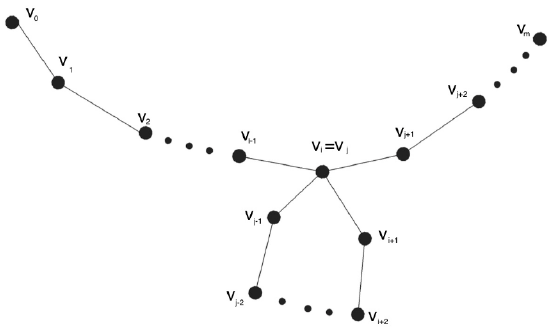
\includegraphics[width = 0.7\linewidth]{CongiungibilitaPasseggiataCammini.PNG}
\end{figure}
\end{center}
\item
Dunque possiamo definire una nuova passeggiata $P \supset P_1 = (y_0, y_1, \dotso, y_i, y_{j+1}, y_{j+2}, \dotso, y_h$ in cui sono stati tolti tutti i vertici tra $v_i$ e $v_j$
\item
In particolare si ha che:
$$ \ell (P_1) = \ell(P_0) - (j - i) < \ell(P_0) \leq \ell(P_1)$$
\item
Ma ciò è impossibile in quanto avevamo dimostrato come $P_0$ fosse il minimo dei cammini possibili.
\item
Abbiamo dimostrato che $P_0$ è un cammino.
\end{itemize}
\item
$C.V.D.$
\end{itemize}
%-------------------------------------------------------------------%
\subsection{Congiungibilità è una relazione di equivalenza}
\textsc{Enunciato:}
\begin{itemize}
\item
La relazione di essere \textbf{congiungibili} (per passeggiata o per cammino) è di \textbf{equivalenza} sui vertici di un grafo.
\end{itemize}
\textsc{Dimostrazione:}
\begin{itemize}
\item
$G = (V,E)$ grafo.
\item
$v,w \in V$, $v \sim w$ se $v$ e $w$ sono  \textbf{congiungibili} in $G$.
\item
$v,w,z \in V$, affinchè sia una relazione deve soddisfare le tre proprietà:
\begin{enumerate}
\item
\textsc{Riflessiva}:
\begin{itemize}
\item
$v \sim v \,\, \forall \, v \in V \, ?$ Vero in quanto $\exists P =(v)$ che è una passeggiata da $v$ in $v$.
\end{itemize}
\item
\textsc{Simmetrica}:
\begin{itemize}
\item
Supponiamo $v \sim w$, ovvero $\exists \,\, (V_0, V_1, \dotso, V_k)$ passeggiata (dove $V_0 = v$ e $V_k = w$).\\
$\implies (V_k, V_{k-1}, \dotso, V_0)$ passeggiata in G (dove $V_k = w$ e $V_0 = v$).\\
$\implies w \sim v$
\end{itemize}
\item
\textsc{Transitiva}:
\begin{itemize}
\item
Supponiamo $v \sim w$ e $w \sim z$, dunque esistono due passeggiate in $G$ tali che:
\begin{itemize}
\item
$P_1 = (v_0 = v, v_1, \,\dotso, v_n = w)$
\item
$P_2 = (y_0 = w, y_1, \,\dotso, y_h = z)$
\end{itemize}
\begin{center}
\begin{figure}[h]
\centering
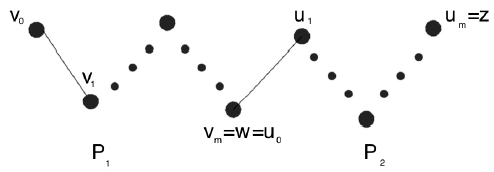
\includegraphics[width = 0.5\linewidth]{CongiungibilitaRelazioneEquivalenza}
\end{figure}
\end{center}
\item
Si può dunque definire una terza passeggiata in $G$:
$$ (v_0 = v, v_1, \dotso, v_k = w = y_0, y_1, \dotso, y_h)$$
\\
$\implies v \sim z$
\end{itemize}
\end{enumerate}
\item
$C.V.D.$
\end{itemize}
%-------------------------------------------------------------------%
\subsection{Relazione fondamentale tra gradi e numero di lati di un grafo finito}
\textsc{Enunciato:}
\begin{itemize}
\item
Sia $G = (V,E)$ un grafo \textbf{finito}, allora:
$$\displaystyle{\sum_{v \in V} deg_G (v) = 2\,|E|}$$
\end{itemize}
\textsc{Dimostrazione:}
\begin{itemize}
\item
Siano $(v_1, \,\dotso,v_n)$ i \textbf{vertici} di $G$ e siano $(e_1, \,\dotso, e_k)$ i \textbf{lati} di $G$.
\item
Per ogni $i \in \{1,\,\dotso, n\}$ e per ogni $j \in \{1,\,\dotso, k\}$, definiamo $m_{i,j} \in \{0,1\}$ come segue:
$$m_{i,j} \begin{cases} 0 \textrm{ se } v_i \neq e_j \\ 1 \textrm{ se } v_i = e_j \end{cases}$$
\item
Prendiamo un piano cartesiano: lungo le $x$ scorre l'indice $i$ e lungo le $y$ scorre l'indice $j$. 
\item
Vale allora:
$$\displaystyle{\sum_{j = 1}^{k} \left(\sum_{i = 1}^{n} m_{i,j} \right) = \sum_{i = 1}^{n} \left(\sum_{j = 1}^{k} m_{i,j} \right)}
$$
\item
Dove il primo membro ha il seguente significato:
\begin{itemize}
\item
$\displaystyle{\sum_{i = 1}^{n} m_{i,j}}$ è il numero di vertici di un lato, che è sempre $2$ (la $j$ è bloccata).
\item
$\displaystyle{\sum_{j = 1}^{k} \left(\sum_{i = 1}^{n} m_{i,j}\right)}$ si sommano $k$ volte ($j \in \{1,\,\dotso,k\}$) il numero di vertici per ciascun lato.
\item
Si ottiene quindi che il primo membro può essere riscritto come:
$$\displaystyle{\sum_{j = 1}^{k} \left(\sum_{i = 1}^{n} m_{i,j}\right) = 2k}$$
\end{itemize}
\item
Mentre il secondo membro ha il seguente significato:
\begin{itemize}
\item
$\displaystyle{\sum_{j = 1}^{k} m_{i,j}}$ è la somma dei numeri su una colonna, posto fisso $i$ per via della sommatoria che precede questa.
\item
$\displaystyle{\sum_{i = 1}^{n} \left(\sum_{j = 1}^{k} m_{i,j}\right)}$ risulta essere la somma dei valori ottenuti sommando i valori di ciascuna colonna.
\item
Ma la prima sommatoria non è altro che la sommatoria di $1$ se un lato entra o esce da un determianto i-esimo vertice, o $0$ se ciò non accade.
\item
Questa somma non è altro che il numero di lati che incontrano tale vertice.
\item
Si può quindi scrivere il primo membro in questo modo:
$$\displaystyle{\sum_{i = 1}^{n} \left(deg_G (v_i)\right)}$$
\end{itemize}
\item
Dunque si ha che:
\begin{equation}
\begin{split}
\sum_{j = 1}^{k} \left(\sum_{i = 1}^{n} m_{i,j} \right) &= \sum_{i = 1}^{n} \left(\sum_{j = 1}^{k} m_{i,j} \right) \\
\sum_{j = 1}^{k} 2 \quad \quad &= \quad \quad \sum_{i = 1}^{n} deg_G (v_i)\\
2k \quad \quad &= \quad \quad \sum_{i = 1}^{n} deg_G (v_i) \\
2\,|E| \quad \quad &= \quad \quad \sum_{i = 1}^{n} deg_G (v_i)
\notag
\end{split}
\end{equation}
\item
$C.V.D$
\end{itemize}
%-------------------------------------------------------------------%
\subsection{Lemma delle strette di mano}
\textsc{Enunciato:}
\begin{itemize}
\item
In un grafo \textbf{finito}, il \textbf{numero di vertici} con \textbf{grado dispari} è \textbf{pari}.
\end{itemize}
\textsc{Dimostrazione:}
\begin{itemize}
\item
$G = (V,E)$ finito:
\begin{equation}
\begin{split}
\displaystyle{\underbrace{2\,|E|}_{\textrm{pari}}} &= \displaystyle{\sum_{v \in V} deg_G(v)} \\
&= \underbrace{\sum_{v \in V} deg_G(v)}_{deg_G(v) \textrm { pari}} \,\,\,\,\, + \,\,\,\,\, \underbrace{\sum_{v \in V} deg_G(v)}_{deg_G(v) \textrm { dispari}} \\
\textrm{numero pari} &= \textrm{numero pari} \implies \textrm{numero pari} 
\end{split}
\end{equation}
\end{itemize}
%-------------------------------------------------------------------%
\subsection{Teorema di caratterizzazione degli alberi finiti}
\textsc{Enunciato:}
\begin{itemize}
\item
Sia $T=(V,E)$ un grafo \textbf{finito}, ovvero $|V|$ è finita.
\item
Le seguenti affermazioni sono equivalenti:
\begin{enumerate}
\item
$T$ è un \textbf{albero}.
\item
$T$ è \textbf{connesso} e vale la seguente \textbf{formula di Eulero}:
$$\displaystyle{|V| - 1 =  |E|  = \frac{1}{2} \sum_{v \in V} deg_T(v)}$$
\end{enumerate}
\textsc{Enunciato:}
\begin{itemize}
\item
$1. \implies 2.$
\begin{itemize}
\item
$T$ è un albero, dunque $T$ è connesso per definizione di albero.
\item
Dobbiamo provare la formula di Eulero.
\item
Procediamo per induzione (1° forma) sul numero di vertici di $T$:
\begin{itemize}
\item
\textbf{Base dell'induzione}: $|V(T)| = 1$, questo implica che $|E(T)| = 0$, dunque:
\begin{equation}
\begin{split}
|V| - 1 &= |E| \\
1 - 1 &= 0
\end{split}
\end{equation}
\item
La base dell'induzione è verificata.
\item
 $|V(T)| \implies |V(T)|$ con $|V(T)| \geq 2$ (\textbf{passo induttivo}).
\item
Sia $T$ un albero (finito) con almeno $2$ vertici ($|V(T)| \geq 2$), allora $T$ possiede almeno 2 foglie (Lemma 20.4).
\item
Sia $v$ una tale foglia.
\item
Poichè $T-v$ è ancora un albero, per \textbf{ipotesi induttiva}, $T-v$ soddisfa la formula di Eulero, cioè:
\begin{equation}
\begin{split}
\underbrace{|V(T-v)|}_{V(T)-1} - 1 &= \underbrace{|E(T-v)|}_{|E(T)-1|} \\
|V(T)|-2 &= |E(T)|-1 \\
|V(T)|-1 &= |E(T)|
\end{split}
\end{equation}
\end{itemize}
\item
La prima implicazione è stata dimostrata.
\end{itemize}
\item
$2. \implies 1.$
\begin{itemize}
\item
Sia $T$ un grafo finito, connesso che soddisfa la formula di Eulero, cioè vale la $2.$
\item
Dobbiamo provare che $T$ è un albero.
\item
Procediamo per induzione su $|V(T)|$:
\begin{itemize}
\item
\textbf{Base dell'induzione}: $$|V(T)| = 1 \textrm{, dunque } T \textrm{ è un albero.}$$
\item
Base dell'induzione dimostata.
\item
$|V(T)| \geq 2$, $|V(T)| - 2 \implies |V(T)|$ (\textbf{ipotesi induttiva}).
\item
Dimostriamo che $T$ ha almeno una foglia. 
\item 
Supponiamo che ciò sia falso.
Poichè $T$ è connesso, il $deg_T(v) \geq 2 \,\, \forall v \in V(T)$ dunque:
\begin{equation}
\begin{split}
|V(T)| - 1 &= |E(T)| \\
2\,|V(T)| - 2 &= 2\,|E(T)| = \sum_{v \in V} deg_T(v) \geq \sum_{v \in V} 2 = 2\,|V(T)| \\
\implies 2\,|V(T)| - 2 \geq 2\,|V(T)| \textrm{ che è assurdo.}
\end{split}
\end{equation}
\item
Abbiamo appena dimostrato che $T$ ha \textbf{almeno una foglia}.
\item
Sia dunque $v$ una foglia di $T$.
\item
Osservo che $T-v$ è \textbf{connesso}.
\item
Ricordiamo che: $$|V(T)-1| = |E(T)| \Longleftrightarrow (|V(T)|-1) - 1 = |E(T)| - 1 \Longleftrightarrow |V(T-v)|-1 = |E(T-v)|$$
\item
Per ipotesi induttiva $T-v$ è un albero ($T-v$ è connesso e soddisfa la formula di Eulero).
\item
Supponiamo che $c$ sia un ciclo di $T$ che passa per i vertici $v$ e $w$.
\item
$T-v$ creerebbe un ciclo, ma visto che $T-v$ per ipotesi è un albero, questo implica che non ha cicli, dunque anche $T$ non ha cicli.
$\implies T$ è un albero. 
\end{itemize}
\item
La seconda implicazione è stata dimostrata.
\end{itemize}
\item
Visto che sia la prima che la seconda implicazione sono state dimostrate, abbiamo finito la dimostrazione del teorema.
\end{itemize}
\end{itemize}
%-------------------------------------------------------------------%
\subsection{Teorema esistenza alberi di copertura}
\textsc{Enunciato:}
\begin{itemize}
\item
Ogni grafo \textbf{finito} e \textbf{connesso} \textbf{ammette un albero di copertura}.
\end{itemize}
\textsc{Dimostrazione:}
\begin{itemize}
\item
Sia $G$ un grafo finito e connesso.
\item
Scriviamo $G=(V,E)$.
\item
Consideriamo:
$$\mathbb{C} := \{C\,|\,C \textrm{ è un sottografo conneso di } G \textrm{ tale che } V(C) = V(G) \}$$
\item
Osserviamo che $\mathbb{C} \neq \varnothing$ in quanto $G \in \mathbb{C}$.
\item
Definiamo:
$$A := \{|E(C)| \in \mathbb{N} \,|\, C \in \mathbb{C}\} \neq \varnothing \textrm{ in quanto } |E(G)| \in \mathbb{A} $$
\item
Grazie al \textbf{teorema di buon ordinamento} $(\mathbb{N},\leq)\,\, \exists \, \overline{C} \in \mathbb{C}$ tale che:
$$|E(\overline{C})| \leq |E(C)| \quad \forall \, C \in \mathbb{C}$$ 
\item
Poichè $\overline{C} \in \mathbb{C}$ vale che $V(\overline{C}) = V(G)$.
\item
Dunque per dimostrare che $\bar{C}$ è un albero di copertura di $G$ è sufficiente verificare che $\bar{C}$ è un albero.
\item
Se $\overline{C}$ non fosse un albero, ciò significherebbe che contiene almeno un ciclo, visto che $\overline{C}$ è connesso ma non è un albero.
\item
Se togliessi un lato da $\overline{C}$, quello che ottengo è un grafo connesso senza cicli.
\item
Ma visto che, togliendo un alto, la minimalità del numero di lati di $\overline{C}$ viene a mancare, cioè $|E(\overline{C}-e)| \leq |E(\overline{C})|$, ma questo è \textbf{assurdo} perchè $|E(\overline{C}|$ è il minor numero di lati, definito per costruzione.
\item
Dunque $\overline{C}$ è un albero e in particolare è un \textbf{albero di copertura}.
\end{itemize}
%-------------------------------------------------------------------%
%-------------------------------------------------------------------%
%-------------------------------------------------------------------%
\end{document}